\documentclass{standalone}
\usepackage{tikz}
\usetikzlibrary{patterns, positioning}
\usepackage[sfdefault]{ClearSans} %% option 'sfdefault' activates Clear Sans as the default text font
\usepackage[T1]{fontenc}

\begin{document}
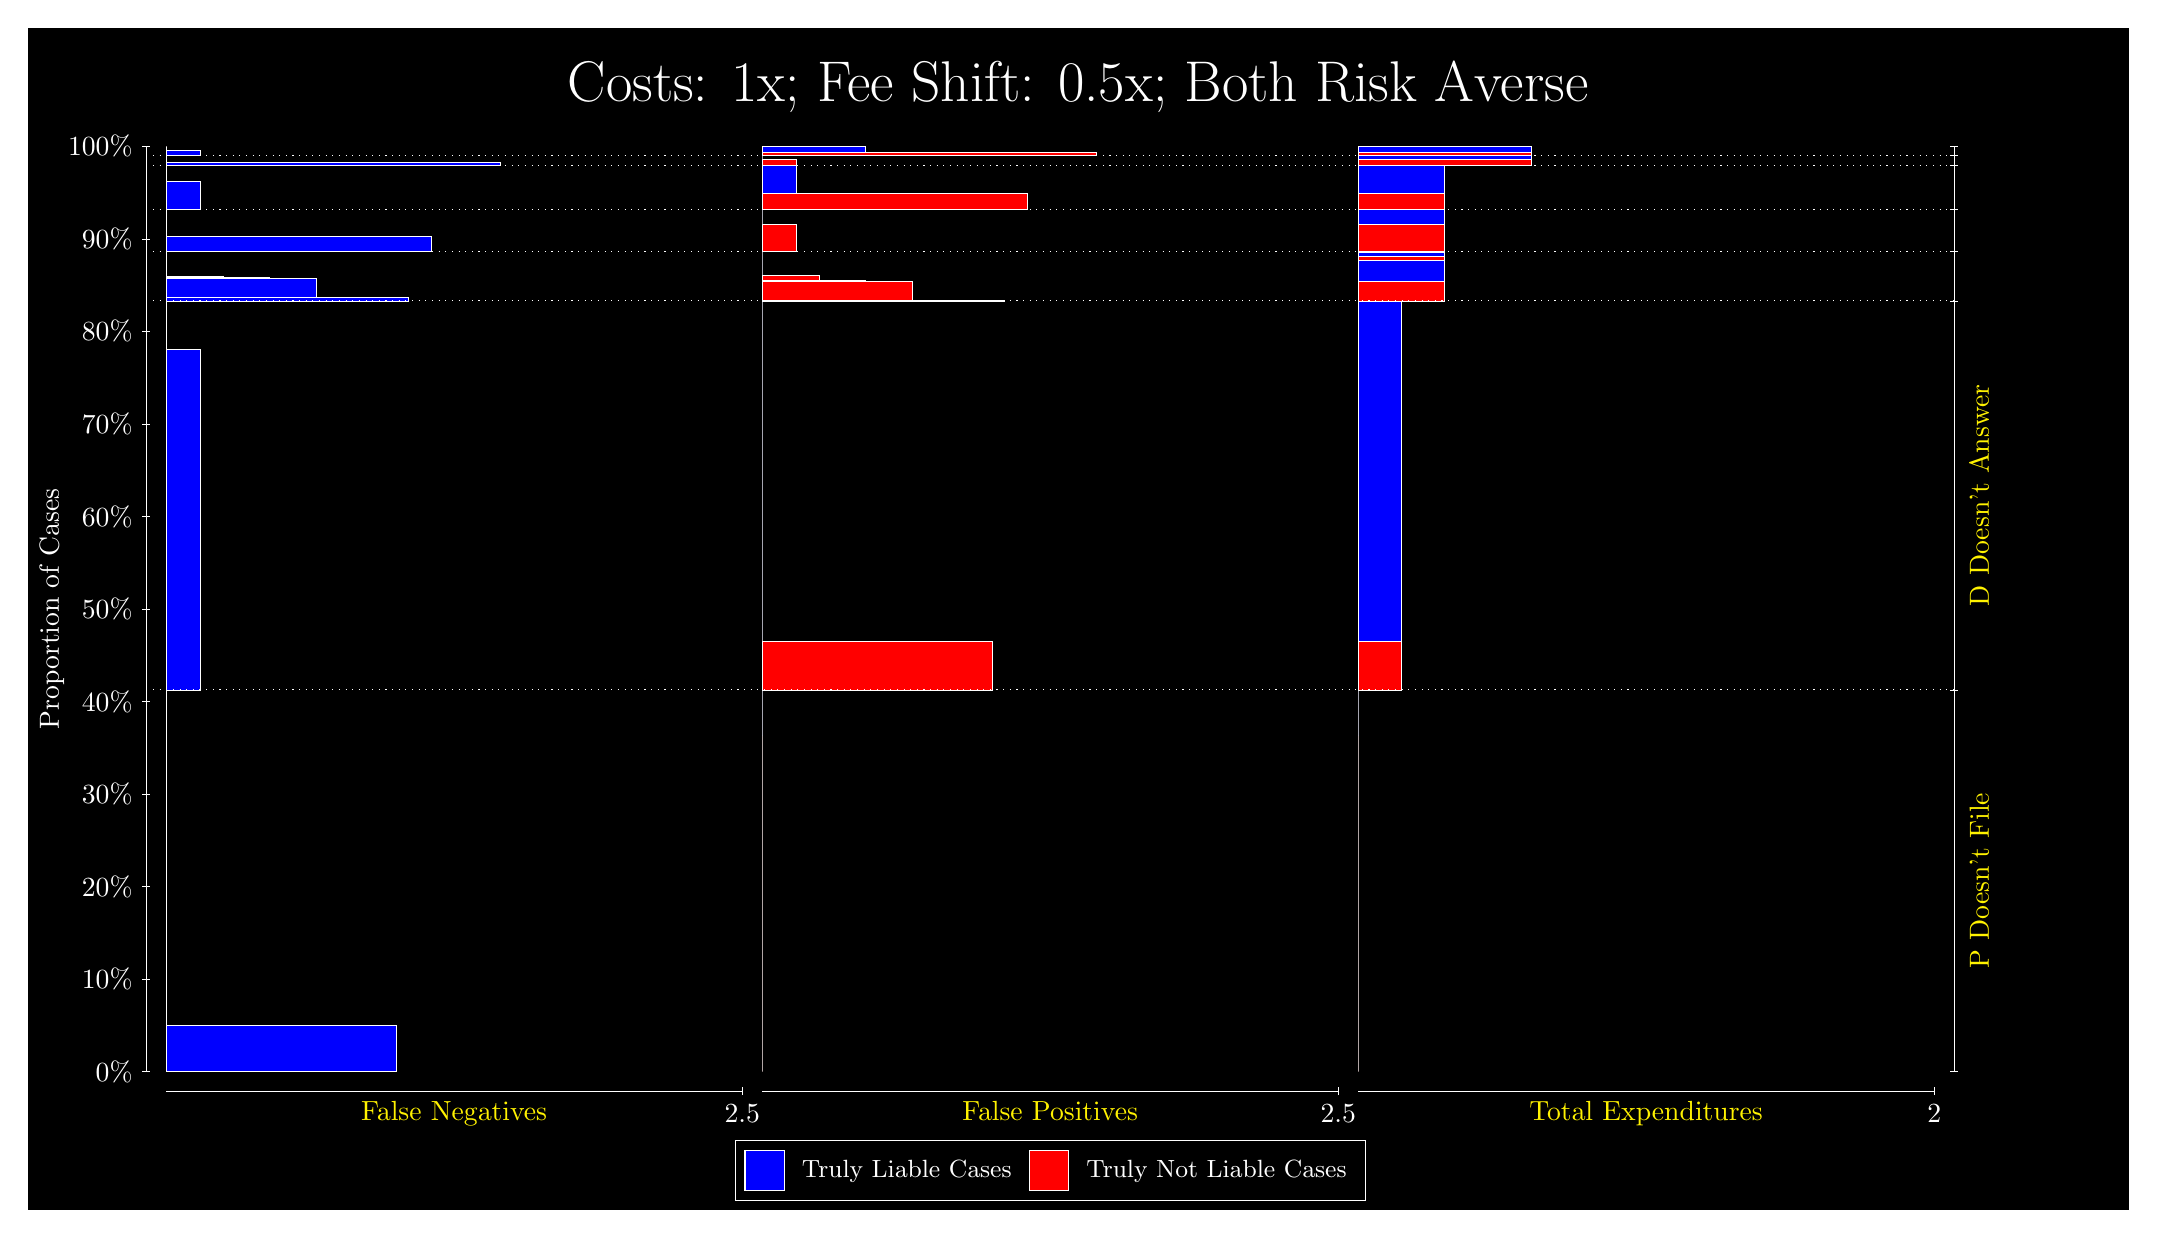
\begin{tikzpicture}
\draw[fill=black] (0,0) rectangle (26.667,15);
\draw[text=white] (0,13.5) rectangle (26.667,15) node[midway] {\huge Costs: 1x; Fee Shift: 0.5x; Both Risk Averse};
\draw[white, very thin] (1.5,1.75) -- (1.5,13.5);
\node[rotate=90, text=white, anchor=center] at (0.3, 7.625) {Proportion of Cases};
\draw[white, very thin] (1.45,1.75) -- (1.55,1.75);
\node[text=white, anchor=east] at (1.45, 1.75) {0\%};
\draw[white, very thin] (1.45,2.925) -- (1.55,2.925);
\node[text=white, anchor=east] at (1.45, 2.925) {10\%};
\draw[white, very thin] (1.45,4.1) -- (1.55,4.1);
\node[text=white, anchor=east] at (1.45, 4.1) {20\%};
\draw[white, very thin] (1.45,5.275) -- (1.55,5.275);
\node[text=white, anchor=east] at (1.45, 5.275) {30\%};
\draw[white, very thin] (1.45,6.45) -- (1.55,6.45);
\node[text=white, anchor=east] at (1.45, 6.45) {40\%};
\draw[white, very thin] (1.45,7.625) -- (1.55,7.625);
\node[text=white, anchor=east] at (1.45, 7.625) {50\%};
\draw[white, very thin] (1.45,8.8) -- (1.55,8.8);
\node[text=white, anchor=east] at (1.45, 8.8) {60\%};
\draw[white, very thin] (1.45,9.975) -- (1.55,9.975);
\node[text=white, anchor=east] at (1.45, 9.975) {70\%};
\draw[white, very thin] (1.45,11.15) -- (1.55,11.15);
\node[text=white, anchor=east] at (1.45, 11.15) {80\%};
\draw[white, very thin] (1.45,12.325) -- (1.55,12.325);
\node[text=white, anchor=east] at (1.45, 12.325) {90\%};
\draw[white, very thin] (1.45,13.5) -- (1.55,13.5);
\node[text=white, anchor=east] at (1.45, 13.5) {100\%};

\draw[white, very thin] (24.457,1.75) -- (24.457,13.5);
\draw[white, very thin] (24.407,1.75) -- (24.507,1.75);
\node[anchor=west] at (24.407, 1.75) {};
\draw[white, very thin] (24.407,6.5975) -- (24.507,6.5975);
\node[anchor=west] at (24.407, 6.5975) {};
\draw[white, very thin] (24.407,11.537) -- (24.507,11.537);
\node[anchor=west] at (24.407, 11.537) {};
\draw[white, very thin] (24.407,12.164) -- (24.507,12.164);
\node[anchor=west] at (24.407, 12.164) {};
\draw[white, very thin] (24.407,12.701) -- (24.507,12.701);
\node[anchor=west] at (24.407, 12.701) {};
\draw[white, very thin] (24.407,13.255) -- (24.507,13.255);
\node[anchor=west] at (24.407, 13.255) {};
\draw[white, very thin] (24.407,13.381) -- (24.507,13.381);
\node[anchor=west] at (24.407, 13.381) {};
\draw[white, very thin] (24.407,13.5) -- (24.507,13.5);
\node[anchor=west] at (24.407, 13.5) {};

\draw[white, very thin, fill=blue] (1.75,1.75) rectangle (4.6775,2.3331);
\draw[white, very thin, fill=red] (1.75,2.3331) rectangle (1.75,6.5975);
\draw[white, very thin, fill=blue] (1.75,6.5975) rectangle (2.1891,10.917);
\draw[white, very thin, fill=red] (1.75,10.917) rectangle (1.75,11.537);
\draw[white, very thin, fill=blue] (1.75,11.537) rectangle (4.8239,11.578);
\draw[white, very thin, fill=blue] (1.75,11.578) rectangle (4.2384,11.585);
\draw[white, very thin, fill=blue] (1.75,11.585) rectangle (3.6529,11.828);
\draw[white, very thin, fill=blue] (1.75,11.828) rectangle (3.0674,11.835);
\draw[white, very thin, fill=blue] (1.75,11.835) rectangle (2.4819,11.844);
\draw[white, very thin, fill=red] (1.75,11.844) rectangle (1.75,12.164);
\draw[white, very thin, fill=blue] (1.75,12.164) rectangle (5.1167,12.359);
\draw[white, very thin, fill=red] (1.75,12.359) rectangle (1.75,12.701);
\draw[white, very thin, fill=blue] (1.75,12.701) rectangle (2.1891,13.051);
\draw[white, very thin, fill=red] (1.75,13.051) rectangle (1.75,13.255);
\draw[white, very thin, fill=blue] (1.75,13.255) rectangle (5.9949,13.3);
\draw[white, very thin, fill=red] (1.75,13.3) rectangle (1.75,13.381);
\draw[white, very thin, fill=blue] (1.75,13.381) rectangle (2.1891,13.456);
\draw[white, very thin, fill=red] (1.75,13.456) rectangle (1.75,13.5);
\draw[white, very thin, fill=red] (9.3189,1.75) rectangle (9.3189,6.0143);
\draw[white, very thin, fill=blue] (9.3189,6.0143) rectangle (9.3189,6.5975);
\draw[white, very thin, fill=red] (9.3189,6.5975) rectangle (12.246,7.2172);
\draw[white, very thin, fill=blue] (9.3189,7.2172) rectangle (9.3189,11.537);
\draw[white, very thin, fill=red] (9.3189,11.537) rectangle (12.393,11.542);
\draw[white, very thin, fill=red] (9.3189,11.542) rectangle (11.807,11.549);
\draw[white, very thin, fill=red] (9.3189,11.549) rectangle (11.222,11.792);
\draw[white, very thin, fill=red] (9.3189,11.792) rectangle (10.636,11.799);
\draw[white, very thin, fill=red] (9.3189,11.799) rectangle (10.051,11.857);
\draw[white, very thin, fill=blue] (9.3189,11.857) rectangle (9.4652,11.866);
\draw[white, very thin, fill=blue] (9.3189,11.866) rectangle (9.3189,12.164);
\draw[white, very thin, fill=red] (9.3189,12.164) rectangle (9.758,12.506);
\draw[white, very thin, fill=blue] (9.3189,12.506) rectangle (9.3189,12.701);
\draw[white, very thin, fill=red] (9.3189,12.701) rectangle (12.686,12.905);
\draw[white, very thin, fill=blue] (9.3189,12.905) rectangle (9.758,13.255);
\draw[white, very thin, fill=red] (9.3189,13.255) rectangle (9.758,13.336);
\draw[white, very thin, fill=blue] (9.3189,13.336) rectangle (9.3189,13.381);
\draw[white, very thin, fill=red] (9.3189,13.381) rectangle (13.564,13.425);
\draw[white, very thin, fill=blue] (9.3189,13.425) rectangle (10.636,13.5);
\draw[white, very thin, fill=red] (16.888,1.75) rectangle (16.888,6.0143);
\draw[white, very thin, fill=blue] (16.888,6.0143) rectangle (16.888,6.5975);
\draw[white, very thin, fill=red] (16.888,6.5975) rectangle (17.437,7.2172);
\draw[white, very thin, fill=blue] (16.888,7.2172) rectangle (17.437,11.537);
\draw[white, very thin, fill=red] (16.888,11.537) rectangle (17.986,11.792);
\draw[white, very thin, fill=blue] (16.888,11.792) rectangle (17.986,12.051);
\draw[white, very thin, fill=red] (16.888,12.051) rectangle (17.986,12.109);
\draw[white, very thin, fill=blue] (16.888,12.109) rectangle (17.986,12.15);
\draw[white, very thin, fill=red] (16.888,12.15) rectangle (17.986,12.157);
\draw[white, very thin, fill=blue] (16.888,12.157) rectangle (17.986,12.164);
\draw[white, very thin, fill=red] (16.888,12.164) rectangle (17.986,12.506);
\draw[white, very thin, fill=blue] (16.888,12.506) rectangle (17.986,12.701);
\draw[white, very thin, fill=red] (16.888,12.701) rectangle (17.986,12.905);
\draw[white, very thin, fill=blue] (16.888,12.905) rectangle (17.986,13.255);
\draw[white, very thin, fill=red] (16.888,13.255) rectangle (19.083,13.336);
\draw[white, very thin, fill=blue] (16.888,13.336) rectangle (19.083,13.381);
\draw[white, very thin, fill=red] (16.888,13.381) rectangle (19.083,13.425);
\draw[white, very thin, fill=blue] (16.888,13.425) rectangle (19.083,13.5);
\draw[white, dotted] (1.5,6.5975) -- (24.457,6.5975);
\draw[white, dotted] (1.5,11.537) -- (24.457,11.537);
\draw[white, dotted] (1.5,12.164) -- (24.457,12.164);
\draw[white, dotted] (1.5,12.701) -- (24.457,12.701);
\draw[white, dotted] (1.5,13.255) -- (24.457,13.255);
\draw[white, dotted] (1.5,13.381) -- (24.457,13.381);
\draw[white, very thin] (1.75,1.5) -- (9.0689,1.5);
\node[text=yellow, anchor=north] at (5.4094, 1.5) {False Negatives};
\draw[white, very thin] (9.0689,1.45) -- (9.0689,1.55);
\node[text=white, anchor=north] at (9.0689, 1.45) {2.5};

\draw[white, very thin] (9.3189,1.5) -- (16.638,1.5);
\node[text=yellow, anchor=north] at (12.978, 1.5) {False Positives};
\draw[white, very thin] (16.638,1.45) -- (16.638,1.55);
\node[text=white, anchor=north] at (16.638, 1.45) {2.5};

\draw[white, very thin] (16.888,1.5) -- (24.207,1.5);
\node[text=yellow, anchor=north] at (20.547, 1.5) {Total Expenditures};
\draw[white, very thin] (24.207,1.45) -- (24.207,1.55);
\node[text=white, anchor=north] at (24.207, 1.45) {2};

\node[text=yellow, centered, rotate=90] at (24.777, 4.1737) {P Doesn't File};
\node[text=yellow, centered, rotate=90] at (24.777, 9.0673) {D Doesn't Answer};






\draw (12.978300999999998,1.5) node[draw=none] (baseCoordinate) {};
\begin{scope}[align=center]
        \matrix[scale=0.5, draw=white, below=0.5cm of baseCoordinate, nodes={draw}, column sep=0.1cm]{
            \node[rectangle, draw, minimum width=0.5cm, minimum height=0.5cm, fill=blue] {}; &
            \node[draw=none, font=\small, text=white] (B) {Truly Liable Cases}; &
            \node[rectangle, draw, minimum width=0.5cm, minimum height=0.5cm, fill=red] {}; &
            \node[draw=none, font=\small, text=white] (B) {Truly Not Liable Cases}; \\
            };
\end{scope}

\end{tikzpicture}
\end{document}